\documentclass[12pt,a4paper]{article}
\usepackage[utf8]{inputenc}
\usepackage[T1]{fontenc}
\usepackage{graphicx}
\usepackage{amsmath,amssymb}
\usepackage{booktabs}
\usepackage{hyperref}
\usepackage{geometry}
\usepackage{float}
\usepackage{caption}
\usepackage{subcaption}
\usepackage{enumitem}
\usepackage{listings}
\usepackage{xcolor}
\usepackage{tikz}
\usetikzlibrary{shapes.geometric, arrows.meta, positioning, fit, backgrounds}

\geometry{margin=2.5cm}

\lstset{
    language=Python,
    basicstyle=\ttfamily\small,
    keywordstyle=\color{blue},
    commentstyle=\color{gray},
    stringstyle=\color{red},
    breaklines=true,
    frame=single,
    numbers=left,
    numberstyle=\tiny\color{gray},
}

\title{Semantic Segmentation for Autonomous Agricultural Robots: \\
\large A U-Net Approach with Auto-Generated Labels}
\author{Prashanna Tiwari}
\date{July 2026}

\begin{document}
\maketitle

\begin{abstract}
This paper presents the development of a semantic segmentation pipeline designed for autonomous navigation in agricultural environments. Inspired by the NATERIDA microbots project---an AI-powered exploration robot capable of environmental monitoring and intelligent data collection---we implement a U-Net convolutional neural network trained on automatically generated pixel-level annotations. The system uses GroundingDINO for open-vocabulary object detection and the Segment Anything Model (SAM) for mask generation, eliminating the need for manual annotation. Data is collected through a simulated Pioneer 3-AT robot performing random-walk exploration in a Webots physics simulator. The model segments scenes into five terrain classes: soil, vegetation, obstacles, pedestrians, and sky. After training for 100 epochs on an NVIDIA GeForce RTX 4060 Laptop GPU with Albumentations-based data augmentation, the system achieves a validation Intersection-over-Union (IoU) of 0.4453 and a Dice coefficient of 0.5497. While these results indicate moderate performance, they demonstrate a viable pipeline for low-cost dataset creation and segmentation model training without manual labeling effort.
\end{abstract}

\tableofcontents
\newpage

%% ============================================================
\section{Introduction}
\label{sec:introduction}
%% ============================================================

Autonomous robots operating in unstructured outdoor environments---such as farms, forests, and disaster zones---must understand the terrain they traverse. Semantic segmentation, the task of classifying every pixel in an image into predefined categories, is fundamental to this capability. A robot that can distinguish soil from vegetation, detect obstacles, and identify pedestrians can make informed navigation decisions without human intervention.

The NATERIDA microbots project~\cite{naterida} demonstrated that a low-cost exploration robot built with an ESP32 microcontroller and off-the-shelf sensors can perform environmental monitoring, plant disease detection, and terrain exploration. NATERIDA uses ResNet-18 for plant disease classification and OpenCV for basic computer vision tasks. However, the project identified a key limitation: the ESP32's compute constraints prevent onboard execution of more sophisticated vision models such as semantic segmentation networks.

This project builds upon that foundation by developing a semantic segmentation pipeline that could, in principle, be deployed on a more capable compute platform (such as an NVIDIA Jetson) integrated into a robot like NATERIDA. The specific contributions of this work are:

\begin{enumerate}[noitemsep]
    \item A fully automated data collection and labeling pipeline using Webots simulation, GroundingDINO, and SAM.
    \item A U-Net segmentation model trained with Albumentations-based augmentation on five terrain classes.
    \item An active segmentation controller that loads the trained model and performs real-time pixel-wise classification on the robot's live camera feed during simulation, demonstrating the model's capability in a simulated deployment scenario.
    \item An evaluation framework reporting IoU and Dice metrics across training and validation splits.
\end{enumerate}

The remainder of this paper is organized as follows: Section~\ref{sec:related} reviews related work, Section~\ref{sec:architecture} describes the system architecture, Section~\ref{sec:mathematical} presents the mathematical foundations, Section~\ref{sec:implementation} details the implementation, Section~\ref{sec:results} presents experimental results, and Sections~\ref{sec:limitations}--\ref{sec:conclusion} discuss limitations, future work, and conclusions.

%% ============================================================
\section{Related Work}
\label{sec:related}
%% ============================================================

\subsection{Semantic Segmentation Architectures}

Semantic segmentation has evolved significantly since the introduction of Fully Convolutional Networks (FCNs) by Long et al.~\cite{long2015}. The U-Net architecture, proposed by Ronneberger et al.~\cite{ronneberger2015} for biomedical image segmentation, introduced an encoder-decoder structure with skip connections that proved highly effective for pixel-wise classification tasks. More recent architectures include DeepLabv3+~\cite{chen2018} which uses atrous spatial pyramid pooling, and SegFormer~\cite{xie2021} which employs transformer-based encoders.

For this project, we chose U-Net because of its simplicity, well-understood training dynamics, and strong performance on relatively small datasets---a practical constraint given our data collection approach.

\subsection{Auto-Labeling with Foundation Models}

Manual annotation of segmentation masks is time-consuming and error-prone. Recent work on text-prompted detection (GroundingDINO~\cite{liu2023grounding}) and universal segmentation (SAM~\cite{kirillov2023}) has enabled automated annotation pipelines. These tools allow researchers to generate pixel-level labels from text descriptions without manual intervention, though the quality depends on the clarity of the text prompts and the diversity of the training data for the foundation models.

\subsection{Robots in Agricultural Settings}

The NATERIDA microbots project~\cite{naterida} demonstrated a practical approach to building exploration robots on a limited budget (under \$60). Their system integrates an ESP32, multiple environmental sensors (DHT11, MQ2, LDR, MPU6050), and a ResNet-18 classifier for plant disease detection. The project highlights the gap between what is computationally feasible on microcontrollers and what is needed for advanced vision tasks---a gap that this segmentation work aims to address for future integration.

%% ============================================================
\section{System Architecture}
\label{sec:architecture}
%% ============================================================

The overall pipeline consists of three stages: data collection, auto-labeling, and model training. Figure~\ref{fig:simulation} shows the Webots simulation environment used for data collection, and Figure~\ref{fig:architecture} illustrates the system flow.

\begin{figure}[H]
\centering
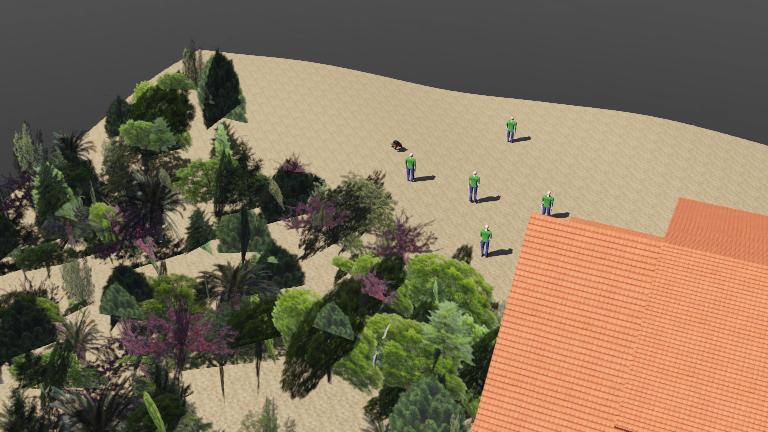
\includegraphics[width=0.85\textwidth]{figures/simulation.jpg}
\caption{Webots simulation environment featuring a Pioneer 3-AT robot navigating through terrain with buildings, vegetation, and pedestrians. The robot is equipped with a camera and lidar sensor for data collection.}
\label{fig:simulation}
\end{figure}

\begin{figure}[H]
\centering
\fbox{\parbox{0.9\textwidth}{\centering
\textbf{System Architecture Overview}\\[10pt]
\texttt{Webots Simulator} $\rightarrow$ \texttt{Data Collection} $\rightarrow$ \texttt{GroundingDINO + SAM} $\rightarrow$ \texttt{Auto-Labeling} $\rightarrow$ \texttt{Albumentations Augmentation} $\rightarrow$ \texttt{U-Net Training} $\rightarrow$ \texttt{Segmentation Model}
}}
\caption{High-level system architecture showing the three-stage pipeline.}
\label{fig:architecture}
\end{figure}

\subsection{U-Net Architecture}

The segmentation model follows the U-Net architecture proposed by Ronneberger et al.~\cite{ronneberger2015}, adapted for our five-class terrain segmentation task. Figure~\ref{fig:unet} shows the complete network structure.

\begin{figure}[H]
\centering
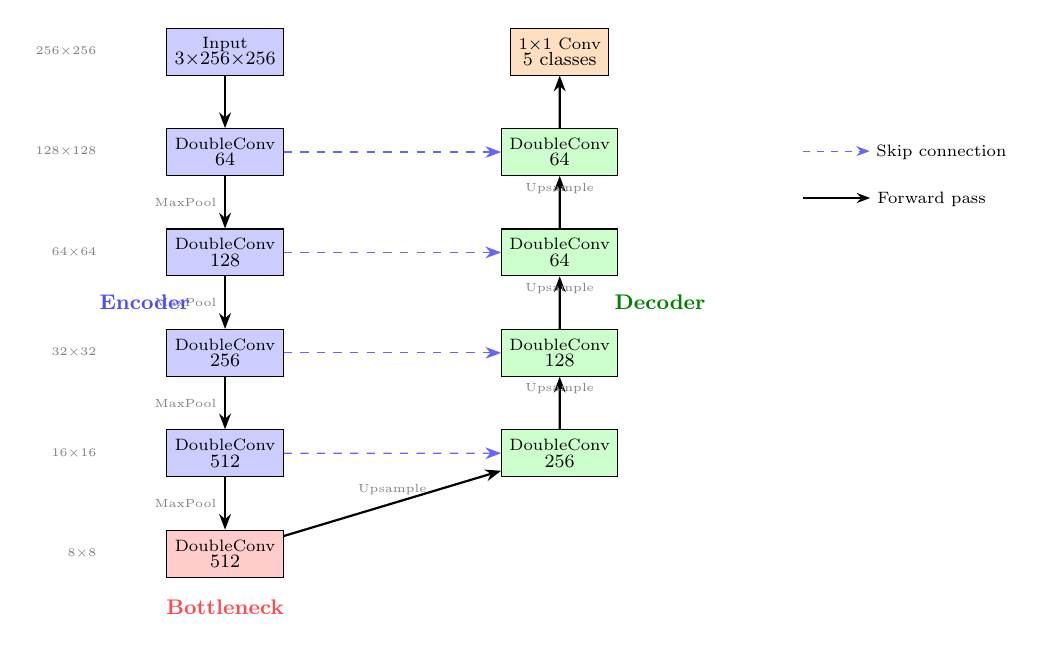
\begin{tikzpicture}[
    scale=0.85, transform shape,
    block/.style={rectangle, draw, minimum width=1.1cm, minimum height=0.7cm, align=center, font=\scriptsize},
    encoder/.style={block, fill=blue!20},
    decoder/.style={block, fill=green!20},
    bottleneck/.style={block, fill=red!20},
    output/.style={block, fill=orange!25},
    pool/.style={font=\tiny, color=gray},
    upsample/.style={font=\tiny, color=gray},
    skip/.style={-{Stealth[length=2mm]}, dashed, color=blue!60},
    arrow/.style={-{Stealth[length=2mm]}, thick},
]

% Encoder path
\node[encoder] (e0) at (0, 0) {Input\\[-1pt]\footnotesize 3$\times$256$\times$256};
\node[encoder] (e1) at (0, -1.5) {DoubleConv\\[-1pt]\footnotesize 64};
\node[encoder] (e2) at (0, -3.0) {DoubleConv\\[-1pt]\footnotesize 128};
\node[encoder] (e3) at (0, -4.5) {DoubleConv\\[-1pt]\footnotesize 256};
\node[encoder] (e4) at (0, -6.0) {DoubleConv\\[-1pt]\footnotesize 512};

% Bottleneck
\node[bottleneck] (b) at (0, -7.5) {DoubleConv\\[-1pt]\footnotesize 512};

% Decoder path
\node[decoder] (d4) at (5, -6.0) {DoubleConv\\[-1pt]\footnotesize 256};
\node[decoder] (d3) at (5, -4.5) {DoubleConv\\[-1pt]\footnotesize 128};
\node[decoder] (d2) at (5, -3.0) {DoubleConv\\[-1pt]\footnotesize 64};
\node[decoder] (d1) at (5, -1.5) {DoubleConv\\[-1pt]\footnotesize 64};

% Output
\node[output] (out) at (5, 0) {1$\times$1 Conv\\[-1pt]\footnotesize 5 classes};

% Encoder arrows (downsampling)
\draw[arrow] (e0) -- node[pool, left] {} (e1);
\draw[arrow] (e1) -- node[pool, left] {MaxPool} (e2);
\draw[arrow] (e2) -- node[pool, left] {MaxPool} (e3);
\draw[arrow] (e3) -- node[pool, left] {MaxPool} (e4);
\draw[arrow] (e4) -- node[pool, left] {MaxPool} (b);

% Bottleneck to decoder
\draw[arrow] (b) -- node[upsample, above] {Upsample} (d4);

% Decoder arrows (upsampling)
\draw[arrow] (d4) -- node[upsample, above] {Upsample} (d3);
\draw[arrow] (d3) -- node[upsample, above] {Upsample} (d2);
\draw[arrow] (d2) -- node[upsample, above] {Upsample} (d1);
\draw[arrow] (d1) -- (out);

% Skip connections
\draw[skip] (e4) -- (d4);
\draw[skip] (e3) -- (d3);
\draw[skip] (e2) -- (d2);
\draw[skip] (e1) -- (d1);

% Labels
\node[font=\small\bfseries, color=blue!70] at (-1.2, -3.75) {Encoder};
\node[font=\small\bfseries, color=green!50!black] at (6.5, -3.75) {Decoder};
\node[font=\small\bfseries, color=red!70] at (0, -8.3) {Bottleneck};

% Resolution annotations
\node[font=\tiny, color=gray, anchor=east] at (-1.8, 0) {256$\times$256};
\node[font=\tiny, color=gray, anchor=east] at (-1.8, -1.5) {128$\times$128};
\node[font=\tiny, color=gray, anchor=east] at (-1.8, -3.0) {64$\times$64};
\node[font=\tiny, color=gray, anchor=east] at (-1.8, -4.5) {32$\times$32};
\node[font=\tiny, color=gray, anchor=east] at (-1.8, -6.0) {16$\times$16};
\node[font=\tiny, color=gray, anchor=east] at (-1.8, -7.5) {8$\times$8};

% Legend
\node[font=\scriptsize, anchor=west] at (8.5, -1.5) {\tikz\draw[skip] (0,0) -- (1,0); Skip connection};
\node[font=\scriptsize, anchor=west] at (8.5, -2.2) {\tikz\draw[arrow] (0,0) -- (1,0); Forward pass};

\end{tikzpicture}
\caption{U-Net architecture used in this work, based on Ronneberger et al.~\cite{ronneberger2015}. The encoder (left) progressively downsamples the input through four levels of double convolutions and max pooling. The decoder (right) recovers spatial resolution through bilinear upsampling and concatenation with skip connections from the corresponding encoder level. The bottleneck at the lowest resolution captures the most abstract features. The final $1 \times 1$ convolution maps 64 feature channels to 5 class logits.}
\label{fig:unet}
\end{figure}

The network follows a symmetric encoder-decoder structure with four resolution levels. Each encoder block consists of two $3 \times 3$ convolutions followed by batch normalization and ReLU activation. Max pooling with a $2 \times 2$ kernel halves the spatial dimensions at each level while doubling the channel count (64 $\rightarrow$ 128 $\rightarrow$ 256 $\rightarrow$ 512). The bottleneck operates at $16 \times$ downsampling with 512 channels.

In the decoder, bilinear upsampling restores spatial resolution, and skip connections concatenate encoder features with decoder features at the same resolution level. This allows the network to recover fine spatial details that would otherwise be lost during downsampling---a key insight of the U-Net design~\cite{ronneberger2015}. The final $1 \times 1$ convolution produces per-pixel logits over the five terrain classes.

\subsection{Data Collection Module}

Data is collected using Webots~\cite{webots}, an open-source robot simulation platform that provides physically accurate modeling of robots, sensors, and environments. Webots simulates rigid-body dynamics, sensor noise models, and realistic lighting, making it suitable for generating training data that approximates real-world conditions without the cost and logistical challenges of physical robot deployment.

\subsubsection{Simulation Environment}

The simulated world (Figure~\ref{fig:simulation}) is built using Webots VRML-based world description and includes the following elements:

\begin{itemize}[noitemsep]
    \item \textbf{Terrain:} An uneven terrain surface with sandy soil texture, providing realistic ground appearance for segmentation.
    \item \textbf{Vegetation:} A procedurally generated forest using the Webots \texttt{Forest} proto, creating dense tree and bush coverage.
    \item \textbf{Structures:} A bungalow-style house proto representing man-made obstacles.
    \item \textbf{Dynamic entities:} A pedestrian proto and an animal (horse) proto, adding dynamic elements to the scene.
    \item \textbf{Lighting:} A textured background with directional lighting that creates realistic shadows and brightness variations.
\end{itemize}

\subsubsection{Robot Platform}

The data collection robot is a Pioneer 3-AT, a four-wheel differential-drive mobile robot commonly used in research. The simulated robot is equipped with:

\begin{itemize}[noitemsep]
    \item \textbf{Camera:} A forward-facing RGB camera mounted at height 0.64\,m, capturing 960$\times$720 pixel images at the simulation timestep rate. The camera provides the raw input for segmentation training.
    \item \textbf{Lidar:} A 10-layer scanning lidar mounted at height 0.34\,m, providing 360-degree range measurements used for obstacle avoidance during data collection.
    \item \textbf{GPS:} A global positioning sensor for logging robot trajectory (not used in the segmentation pipeline).
    \item \textbf{Wheels:} Four independent wheels controlled via velocity commands through an L298N-equivalent motor driver interface.
\end{itemize}

\subsubsection{Exploration Strategy}

The robot employs a hybrid exploration strategy to collect diverse training images:

\begin{enumerate}[noitemsep]
    \item \textbf{Random walk:} Eight movement primitives (forward, backward, sharp/gentle left/right turns, spin left/right) are sampled with a constraint that no move repeats more than twice consecutively. Each move persists for 5 seconds, and camera frames are captured every 5--10 seconds. This ensures the robot visits diverse viewpoints and terrain configurations.

    \item \textbf{Lidar-based obstacle avoidance:} The 10-layer lidar range image is partitioned into left, center, and right sectors by dividing the 360-degree scan into three equal arcs. If the average center clearance falls below 1.0\,m, the robot executes a turning maneuver toward the clearer side (left or right), preventing collision and ensuring continuous data collection.
\end{enumerate}

This approach yielded 908 images across varied terrain including sandy ground, vegetation, buildings, pedestrians, and sky. The exploration ran for approximately 75 minutes of simulated time, with the robot covering a trajectory of several hundred meters through the environment.

\subsubsection{Camera Image Pipeline}

At each capture interval, the robot's camera returns a raw BGRA buffer from the Webots physics engine. The processing pipeline converts this to an RGB numpy array, writes it as a PNG file to the dataset directory, and optionally displays a live preview window (when a display server is available). The raw images retain their native 960$\times$720 resolution and are only downsampled to 256$\times$256 during training.

Figure~\ref{fig:seg_both} illustrates the concept of real-time semantic segmentation overlay, where the trained U-Net model processes each camera frame and produces a pixel-wise classification that is blended with the original image for visual inspection.

\subsection{Auto-Labeling Module}

Rather than manually annotating 908 images, we employed a two-stage auto-labeling pipeline:

\begin{enumerate}[noitemsep]
    \item \textbf{GroundingDINO} detects bounding boxes for each class using text prompts (e.g., ``sandy soil ground dirt path'' for soil, ``green vegetation tree bush plant'' for vegetation).
    \item \textbf{SAM (Segment Anything Model)} generates pixel-precise masks within each detected bounding box.
\end{enumerate}

The final mask is a single-channel grayscale image where each pixel value corresponds to a class index (0--4). Heuristic fills are applied: unlabeled pixels in the lower half of the image default to soil (class 0), and unlabeled pixels in the top quarter default to sky (class 4). This process produced 888 matched image-mask pairs.

\subsection{Dataset Visualization}

Figure~\ref{fig:sample} shows a representative example from the collected dataset. The raw camera image (a) captures terrain with buildings, vegetation, and sky. The auto-generated segmentation mask (b) assigns each pixel to one of five terrain classes, displayed with enhanced contrast and class-specific colors for visibility: brown for soil, green for vegetation, red for obstacles, blue for pedestrians, and gray for sky. The color overlay (c) superimposes the enhanced mask onto the original image at $\alpha = 0.45$, enabling visual verification that the auto-labels align with the scene geometry.

\begin{figure}[H]
\centering
\begin{subfigure}[b]{0.3\textwidth}
    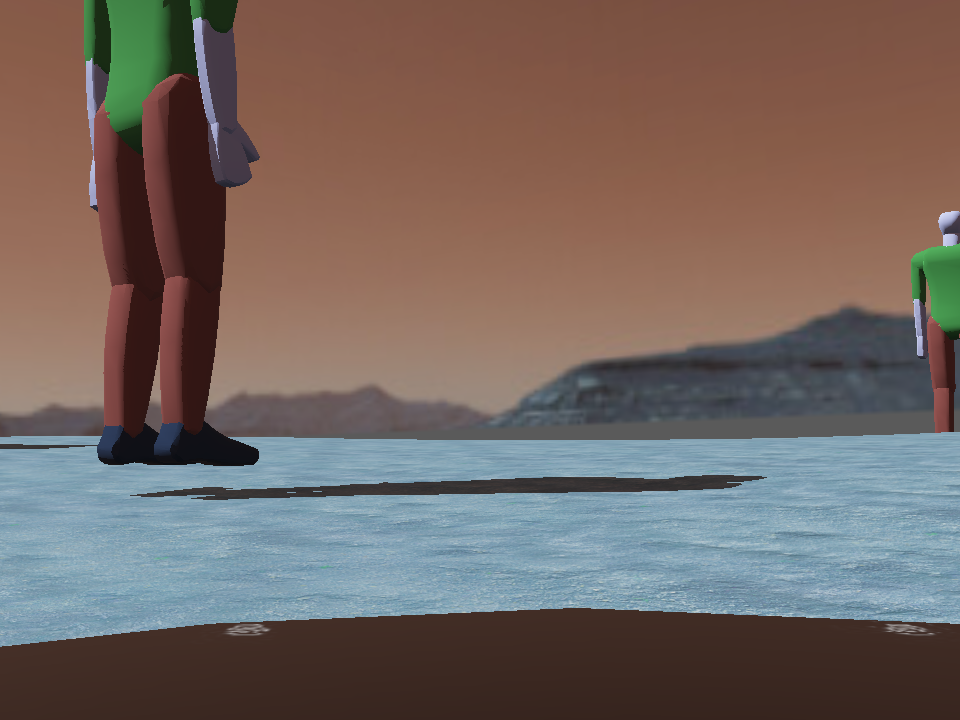
\includegraphics[width=\textwidth]{figures/sample_image.png}
    \caption{Input image}
    \label{fig:sample_img}
\end{subfigure}
\hfill
\begin{subfigure}[b]{0.3\textwidth}
    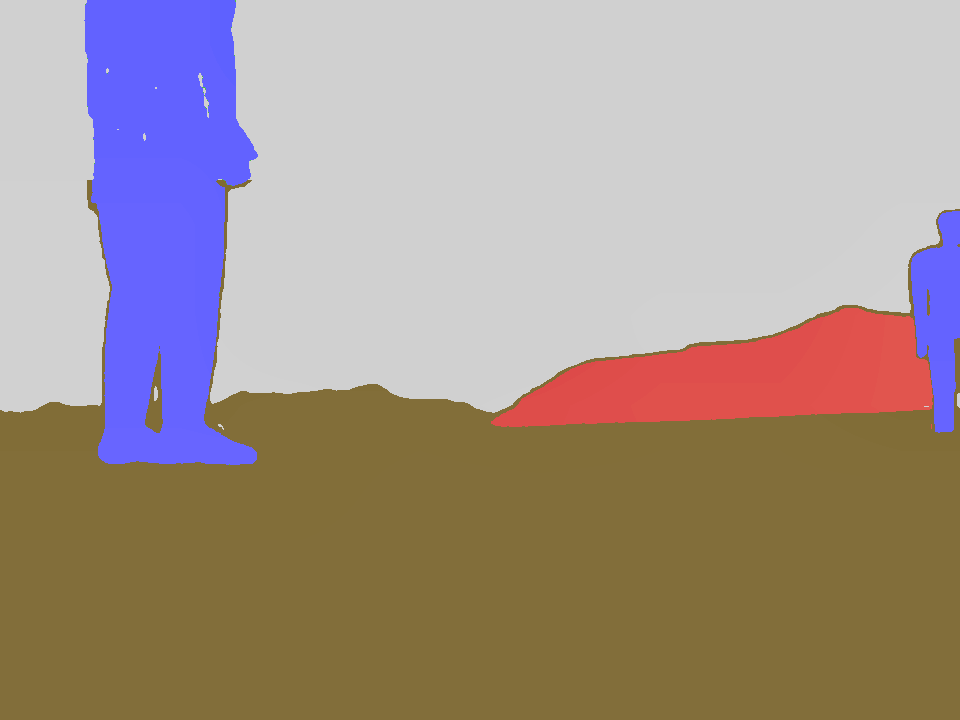
\includegraphics[width=\textwidth]{figures/sample_mask_enhanced.png}
    \caption{Enhanced mask}
    \label{fig:sample_mask}
\end{subfigure}
\hfill
\begin{subfigure}[b]{0.3\textwidth}
    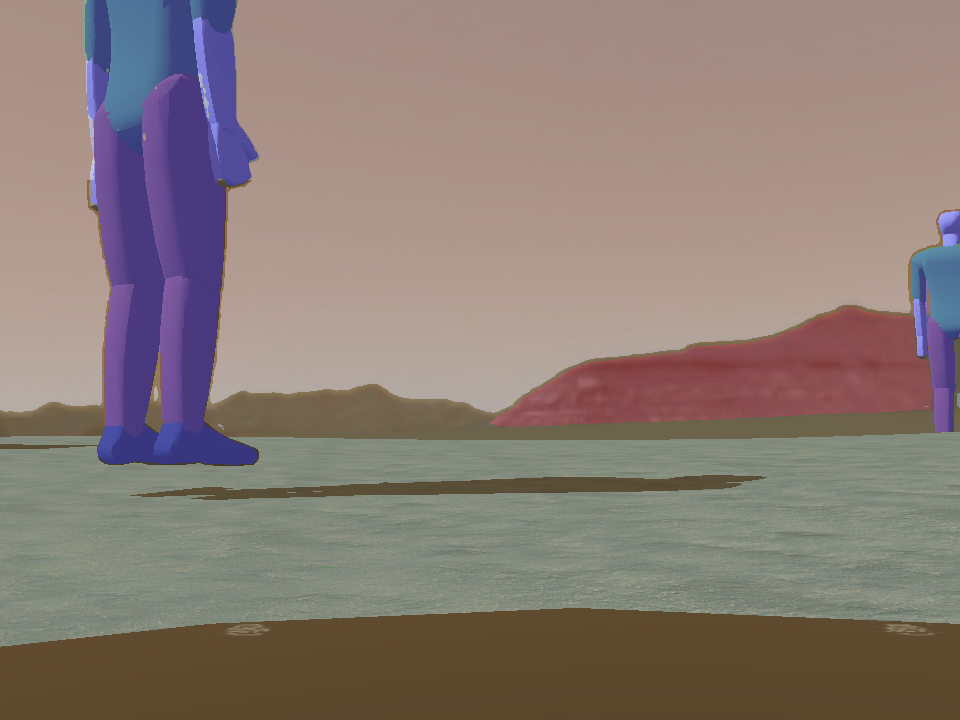
\includegraphics[width=\textwidth]{figures/sample_overlay_final.png}
    \caption{Overlay}
    \label{fig:sample_overlay}
\end{subfigure}
\caption{Dataset sample: (a)~raw 960$\times$720 camera image from the Webots simulation, (b)~auto-generated ground-truth mask with CLAHE contrast enhancement and gamma correction ($\gamma = 0.6$) applied for visibility, (c)~color overlay blending the enhanced mask with the original image for visual verification of label quality.}
\label{fig:sample}
\end{figure}

\subsection{Real-Time Segmentation Pipeline}

Once trained, the U-Net model can process live camera feeds from the robot to produce pixel-wise terrain classification in real time. The active segmentation controller (\texttt{unet.py}) loads the trained checkpoint, initializes the U-Net in evaluation mode, and runs inference on each camera frame received from the Webots simulator. Figure~\ref{fig:segmentation_pipeline} shows the data flow: each RGB frame is normalized and passed through the U-Net encoder-decoder, producing a $5 \times H \times W$ logit tensor. The argmax operation selects the most likely class per pixel, and a color map is applied to create a visual overlay.

\begin{figure}[H]
\centering
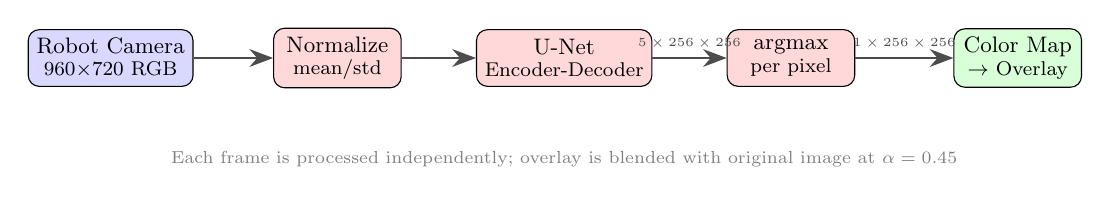
\begin{tikzpicture}[
    scale=0.9, transform shape,
    block/.style={rectangle, draw, rounded corners, minimum width=1.8cm, minimum height=0.8cm, align=center, font=\small},
    camera/.style={block, fill=blue!15},
    model/.style={block, fill=red!15},
    output/.style={block, fill=green!15},
    arrow/.style={-{Stealth[length=3mm]}, thick, color=black!70},
]

\node[camera] (cam) at (0, 0) {Robot Camera\\[-2pt]\footnotesize 960$\times$720 RGB};
\node[model] (norm) at (3.2, 0) {Normalize\\[-2pt]\footnotesize mean/std};
\node[model] (unet) at (6.4, 0) {U-Net\\[-2pt]\footnotesize Encoder-Decoder};
\node[model] (argmax) at (9.6, 0) {argmax\\[-2pt]\footnotesize per pixel};
\node[output] (cmap) at (12.8, 0) {Color Map\\[-2pt]\footnotesize $\rightarrow$ Overlay};

\draw[arrow] (cam) -- (norm);
\draw[arrow] (norm) -- (unet);
\draw[arrow] (unet) -- node[above, font=\tiny] {$5 \times 256 \times 256$} (argmax);
\draw[arrow] (argmax) -- node[above, font=\tiny] {$1 \times 256 \times 256$} (cmap);

\node[font=\scriptsize, color=gray, anchor=north] at (6.4, -1.2) {Each frame is processed independently; overlay is blended with original image at $\alpha = 0.45$};

\end{tikzpicture}
\caption{Real-time segmentation data flow. Each camera frame passes through normalization, U-Net inference, class assignment via argmax, and color mapping to produce a segmentation overlay.}
\label{fig:segmentation_pipeline}
\end{figure}

\subsubsection{Controller Design}

The active segmentation controller operates as follows during each simulation timestep:

\begin{enumerate}[noitemsep]
    \item The robot continues its random exploration strategy (same as data collection), choosing movement primitives and avoiding obstacles via lidar.
    \item At each timestep, the controller reads the camera's BGRA buffer and converts it to RGB for inference.
    \item The frame is resized to 256$\times$256, normalized with ImageNet statistics (mean $= [0.485, 0.456, 0.406]$, std $= [0.229, 0.224, 0.225]$), and passed through the U-Net as a $1 \times 3 \times 256 \times 256$ tensor.
    \item The model outputs a $1 \times 5 \times 256 \times 256$ logit tensor. An \texttt{argmax} along the class dimension produces a $256 \times 256$ prediction map where each pixel value (0--4) corresponds to a terrain class.
    \item The prediction map is color-coded using a fixed palette (brown $=$ soil, green $=$ vegetation, red $=$ obstacle, blue $=$ pedestrian, gray $=$ sky) and blended with the original frame at $\alpha = 0.45$ to produce the segmentation overlay.
    \item Two OpenCV windows are displayed side by side: the raw camera feed with status information, and the segmentation overlay with a class legend.
\end{enumerate}

This setup serves as an initial demonstration of active segmentation in simulation. While the current system does not yet use the segmentation output for navigation decisions, it validates that the trained model can process live camera feeds and produce meaningful pixel-wise classifications. In future work, the segmentation output could be used for obstacle avoidance, path planning, or terrain-adaptive navigation---moving beyond the random walk strategy used here.

\subsubsection{Inference Performance}

Since the simulated camera streams frames to the Python controller via the Webots API, inference runs on the host machine's GPU (NVIDIA RTX 4060) rather than onboard the robot. The U-Net processes each 256$\times$256 frame in approximately 15--30\,ms, depending on GPU load. This is fast enough for near-real-time visualization but would need optimization for a physical robot with limited compute.

For deployment on edge hardware such as the NVIDIA Jetson Nano, the model could be exported to TorchScript or ONNX format and quantized to INT8 precision. The Jetson Nano's 128 CUDA cores can execute a U-Net of this size at approximately 5--10 frames per second at 256$\times$256 resolution, which is sufficient for slow-moving agricultural robots.

\subsubsection{Dual-Window Display}

The controller displays two synchronized OpenCV windows during operation:

\begin{itemize}[noitemsep]
    \item \textbf{Camera window:} Shows the raw RGB camera feed with a text overlay indicating the current movement primitive, the number of saved frames, and the inference time in milliseconds.
    \item \textbf{Segmentation window:} Shows the color-coded prediction overlay blended with the original image, with a class legend in the top-left corner and inference timing at the bottom.
\end{itemize}

Figure~\ref{fig:seg_both} shows both windows displayed simultaneously during an active segmentation run in the Webots simulator.

\begin{figure}[H]
\centering
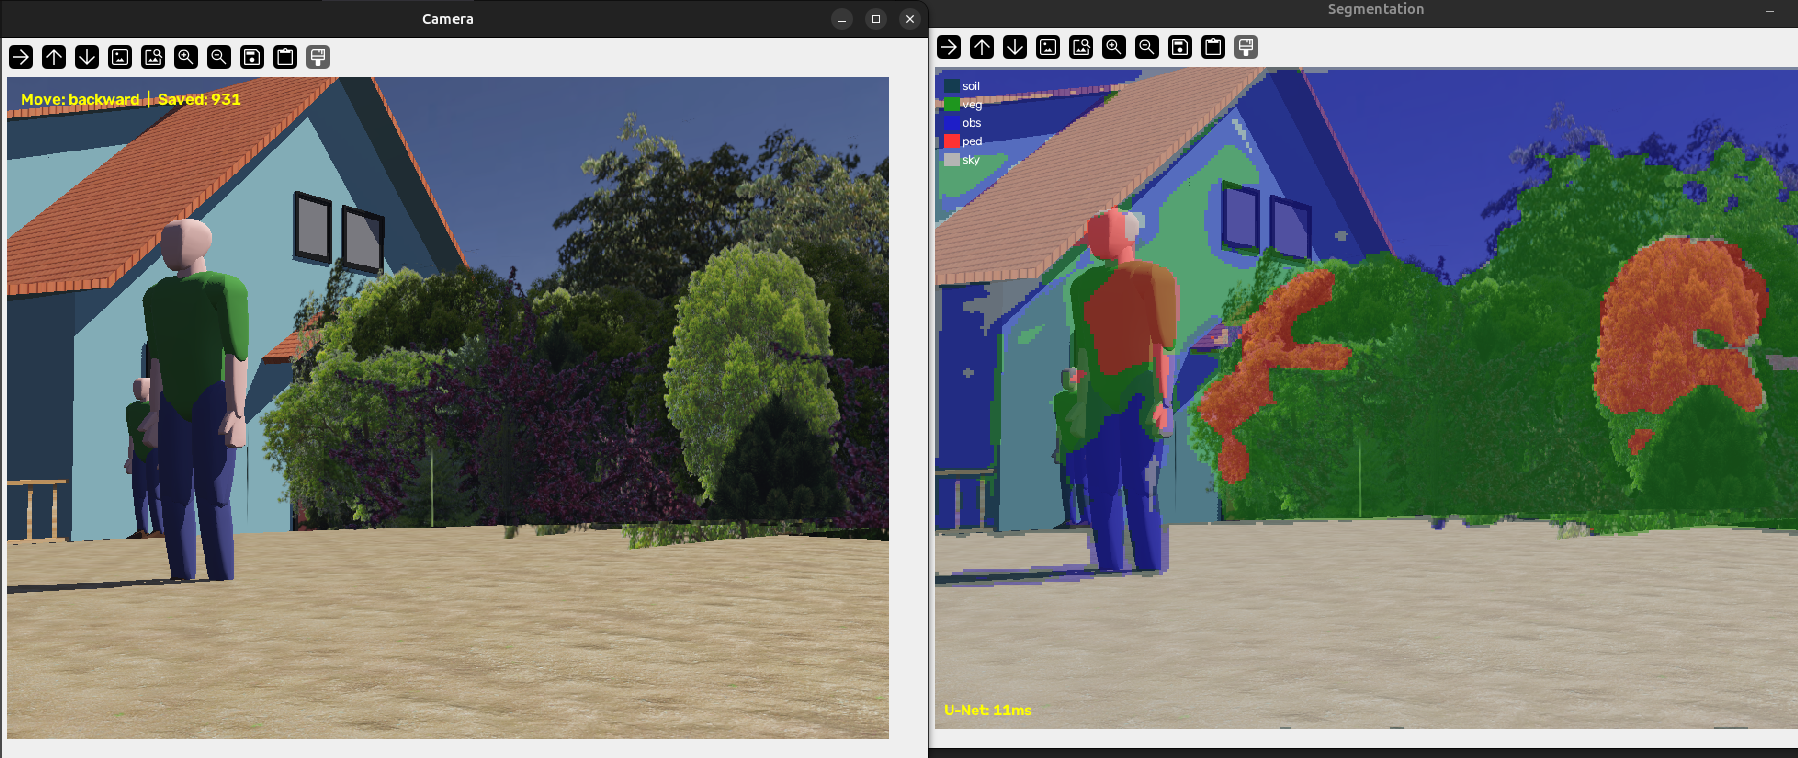
\includegraphics[width=0.95\textwidth]{figures/semantic_seg.png}
\caption{Full active segmentation interface showing both the raw camera feed (left) and the U-Net segmentation overlay (right) displayed simultaneously during Webots simulation.}
\label{fig:seg_both}
\end{figure}

\subsection{Training Module}

The training pipeline uses PyTorch with the following components:
\begin{itemize}[noitemsep]
    \item \textbf{Augmentation:} Albumentations library with 10 transforms (horizontal/vertical flips, affine transforms, color jitter, noise, blur, elastic/grid/optical distortion).
    \item \textbf{Dataset split:} 85\% training (754 images), 15\% validation (134 images), using stratified random splitting.
    \item \textbf{Loss function:} Class-weighted CrossEntropyLoss to handle terrain class imbalance.
    \item \textbf{Optimizer:} AdamW with weight decay $10^{-5}$ and cosine annealing learning rate schedule.
\end{itemize}

%% ============================================================
\section{Mathematical Foundations}
\label{sec:mathematical}
%% ============================================================

This section describes the key mathematical concepts underlying the segmentation pipeline, presented at a level appropriate for a second-year undergraduate student.

\subsection{Convolutional Operations}

The core operation in a CNN is the discrete convolution. For a 2D input feature map $X$ and a kernel $K$ of size $k \times k$, the output at position $(i,j)$ is:

\begin{equation}
    (X * K)(i,j) = \sum_{m=0}^{k-1} \sum_{n=0}^{k-1} X(i+m, j+n) \cdot K(m,n)
\end{equation}

In practice, we learn the kernel weights $K$ through backpropagation. A $3 \times 3$ convolution with padding 1 preserves the spatial dimensions of the input.

\subsection{U-Net Encoder-Decoder Structure}

The U-Net consists of a contracting path (encoder) and an expanding path (decoder). At each level $l$ of the encoder, the feature map $F_l$ is computed as:

\begin{equation}
    F_l = \text{ReLU}\bigl(\text{BN}(\text{Conv}(F_{l-1}, W_l))\bigr)
\end{equation}

where $\text{BN}$ denotes batch normalization and $W_l$ are the learnable weights. After each double convolution, max pooling with a $2 \times 2$ kernel reduces spatial dimensions by half:

\begin{equation}
    F_{l+1} = \text{MaxPool}(F_l)
\end{equation}

In the decoder, the feature map is upsampled and concatenated with the corresponding encoder feature map (skip connection):

\begin{equation}
    D_l = \text{Conv}\bigl(\text{Concat}(U_l, F_l)\bigr)
\end{equation}

where $U_l$ is the upsampled feature map from the previous decoder level. The skip connections allow the decoder to recover fine spatial details lost during downsampling.

\subsection{Cross-Entropy Loss}

For a pixel-level classification problem with $C$ classes, the cross-entropy loss for a single pixel with predicted logits $z_c$ and ground-truth class $t$ is:

\begin{equation}
    \mathcal{L}_{\text{CE}} = -\sum_{c=1}^{C} w_c \cdot \mathbb{1}[t = c] \cdot \log\left(\frac{e^{z_c}}{\sum_{j=1}^{C} e^{z_j}}\right)
\end{equation}

The softmax operation $\sigma(z_c) = \frac{e^{z_c}}{\sum_j e^{z_j}}$ converts logits into a probability distribution over classes. The weights $w_c$ are computed as:

\begin{equation}
    w_c = \frac{N}{C \cdot n_c}
\end{equation}

where $N$ is the total number of pixels, $C$ is the number of classes (5), and $n_c$ is the number of pixels belonging to class $c$. This weighting compensates for class imbalance---for example, soil pixels vastly outnumber pedestrian pixels in our dataset.

\subsection{Evaluation Metrics}

\textbf{Intersection-over-Union (IoU)} for class $c$ measures the overlap between predicted and ground-truth regions:

\begin{equation}
    \text{IoU}_c = \frac{|P_c \cap G_c|}{|P_c \cup G_c|} = \frac{\text{TP}_c}{\text{TP}_c + \text{FP}_c + \text{FN}_c}
\end{equation}

where $P_c$ is the set of pixels predicted as class $c$, $G_c$ is the ground-truth set, TP denotes true positives, FP false positives, and FN false negatives.

\textbf{Dice Coefficient} is a related measure of overlap:

\begin{equation}
    \text{Dice}_c = \frac{2|P_c \cap G_c|}{|P_c| + |G_c|} = \frac{2\,\text{TP}_c}{2\,\text{TP}_c + \text{FP}_c + \text{FN}_c}
\end{equation}

The Dice coefficient ranges from 0 (no overlap) to 1 (perfect overlap) and is more sensitive to small regions than accuracy alone.

\subsection{Data Augmentation as Regularization}

Data augmentation applies random transformations to training samples, effectively expanding the dataset. For a transformation $T$ sampled from a distribution $\mathcal{T}$, the augmented dataset becomes:

\begin{equation}
    \mathcal{D}_{\text{aug}} = \{(T(x_i),\, T(y_i)) \mid (x_i, y_i) \in \mathcal{D},\, T \sim \mathcal{T}\}
\end{equation}

where both the image $x_i$ and its corresponding mask $y_i$ must undergo the same spatial transformation (e.g., rotation, flip) to maintain pixel-level alignment. Photometric transformations (brightness, contrast) are applied only to the image.

%% ============================================================
\section{Implementation Details}
\label{sec:implementation}
%% ============================================================

\subsection{Software Libraries}

The project relies on the following software stack, all running within a Conda environment (\texttt{rl}) on Python 3.10:

\begin{table}[H]
\centering
\caption{Software dependencies and their roles.}
\label{tab:software}
\begin{tabular}{@{}lll@{}}
\toprule
\textbf{Library} & \textbf{Version} & \textbf{Purpose} \\
\midrule
PyTorch & 2.12.1+cu130 & Deep learning framework, GPU acceleration \\
TorchVision & 0.27.1+cu130 & Image utilities \\
Albumentations & 2.0.8 & Data augmentation pipeline \\
OpenCV & 5.0.0 & Image I/O and preprocessing \\
NumPy & 2.2.6 & Array operations \\
Scikit-learn & 1.7.2 & Train/validation splitting \\
SciPy & --- & Morphological mask post-processing \\
GroundingDINO & --- & Text-prompted object detection \\
SAM & --- & Segment Anything Model for mask generation \\
Webots & R2025a & Physics-based robot simulation \\
\bottomrule
\end{tabular}
\end{table}

\subsection{Hardware Resources}

Training was performed on a laptop with the following specifications:

\begin{table}[H]
\centering
\caption{Hardware specifications for model training.}
\label{tab:hardware}
\begin{tabular}{@{}ll@{}}
\toprule
\textbf{Component} & \textbf{Specification} \\
\midrule
GPU & NVIDIA GeForce RTX 4060 Laptop (8\,GB VRAM) \\
CUDA Version & 13.0 \\
CPU & (not critical for this work) \\
RAM & Sufficient for batch size 4 at 256$\times$256 \\
\bottomrule
\end{tabular}
\end{table}

The RTX 4060 Laptop GPU, based on NVIDIA's Ada Lovelace architecture, provides sufficient CUDA cores and VRAM for training a standard U-Net at 256$\times$256 resolution with a batch size of 4. Training 100 epochs on 754 images completed in approximately 15--20 minutes.

\subsection{Data Augmentation Pipeline}

The training augmentation pipeline applies the following transforms in sequence with the listed probabilities:

\begin{table}[H]
\centering
\caption{Data augmentation transforms applied during training.}
\label{tab:augmentation}
\begin{tabular}{@{}lcc@{}}
\toprule
\textbf{Transform} & \textbf{Parameters} & \textbf{Probability} \\
\midrule
HorizontalFlip & --- & 0.5 \\
VerticalFlip & --- & 0.2 \\
RandomRotate90 & --- & 0.3 \\
Affine & translate $\pm$10\%, scale 0.8--1.2$\times$, rotate $\pm$15$^\circ$ & 0.5 \\
RandomBrightnessContrast & brightness/contrast $\pm$0.3 & 0.5 (OneOf) \\
CLAHE & clip\_limit=4.0 & 0.5 (OneOf) \\
RandomGamma & gamma 70--130\% & 0.5 (OneOf) \\
GaussNoise & --- & 0.3 (OneOf) \\
GaussianBlur & kernel 3--5 & 0.3 (OneOf) \\
ElasticTransform & $\alpha$=120, $\sigma$=6 & 0.2 (OneOf) \\
GridDistortion & 5 steps, limit 0.3 & 0.2 (OneOf) \\
OpticalDistortion & distort\_limit=0.2 & 0.2 (OneOf) \\
\bottomrule
\end{tabular}
\end{table}

All augmentations include the corresponding mask transformation for spatial transforms, ensuring pixel-level alignment between image and mask pairs. Validation uses only normalization (mean=[0.485, 0.456, 0.406], std=[0.229, 0.224, 0.225]) with no random augmentation.

\subsection{Training Configuration}

\begin{table}[H]
\centering
\caption{Training hyperparameters.}
\label{tab:hyperparams}
\begin{tabular}{@{}ll@{}}
\toprule
\textbf{Parameter} & \textbf{Value} \\
\midrule
Image resolution & 256$\times$256 \\
Input channels & 3 (RGB) \\
Output classes & 5 (soil, vegetation, obstacle, pedestrian, sky) \\
Batch size & 4 \\
Epochs & 100 \\
Learning rate & $1 \times 10^{-4}$ (initial) \\
LR scheduler & Cosine annealing ($\eta_{\min} = 10^{-6}$) \\
Optimizer & AdamW (weight decay $= 10^{-5}$) \\
Loss function & Weighted CrossEntropyLoss \\
Train/Val split & 85\%/15\% (754/134 images) \\
\bottomrule
\end{tabular}
\end{table}

%% ============================================================
\section{Results and Discussion}
\label{sec:results}
%% ============================================================

\subsection{Training Progress}

Table~\ref{tab:results} presents the training and validation metrics at selected epochs throughout the 100-epoch training run.

\begin{table}[H]
\centering
\caption{Training and validation metrics at selected epochs.}
\label{tab:results}
\begin{tabular}{@{}ccccc@{}}
\toprule
\textbf{Epoch} & \textbf{Train Loss} & \textbf{Val Loss} & \textbf{Val IoU} & \textbf{Val Dice} \\
\midrule
1   & 1.3826 & 1.2112 & 0.2707 & 0.3662 \\
5   & 1.2298 & 1.0600 & 0.3036 & 0.4087 \\
10  & 1.1474 & 0.9291 & 0.3822 & 0.4858 \\
25  & 1.0744 & 0.8996 & 0.3949 & 0.5033 \\
40  & 1.0045 & 0.8516 & 0.4055 & 0.5165 \\
50  & 0.9672 & 0.8467 & 0.3772 & 0.4912 \\
65  & 0.9455 & 0.7993 & 0.4046 & 0.5174 \\
75  & 0.9027 & 0.7813 & \textbf{0.4411} & \textbf{0.5497} \\
80  & 0.8937 & 0.7699 & 0.4317 & 0.5417 \\
100 & 0.8737 & 0.7608 & 0.4245 & 0.5379 \\
\bottomrule
\end{tabular}
\end{table}

\subsection{Key Observations}

\begin{enumerate}[noitemsep]
    \item \textbf{Steady loss decrease:} Both training and validation loss decrease consistently throughout training, indicating the model is learning without severe overfitting. The training loss drops from 1.38 to 0.87, while validation loss drops from 1.21 to 0.76.

    \item \textbf{Peak performance at epoch 75:} The best validation IoU (0.4411) and Dice (0.5497) occur at epoch 75, after which performance plateaus or slightly degrades. The best model checkpoint is saved at this point.

    \item \textbf{Class imbalance impact:} The class weight computation reveals significant imbalance: vegetation receives the highest weight (3.101$\times$) while sky receives the lowest (0.128$\times$). This suggests soil and sky dominate the dataset, while vegetation and obstacle classes are underrepresented.

    \item \textbf{Moderate IoU:} An IoU of 0.4453 is moderate for a 5-class terrain segmentation task. This is expected given the dataset size (888 images), the reliance on auto-generated labels (which contain noise), and the relatively simple U-Net architecture. State-of-the-art models on benchmark datasets like Cityscapes typically achieve IoU $> 0.70$, but they are trained on tens of thousands of manually annotated images.
\end{enumerate}

\subsection{Comparison with NATERIDA}

The NATERIDA microbots project~\cite{naterida} achieved plant disease classification using ResNet-18, which is a simpler task (image-level classification) compared to pixel-level segmentation. Our work extends the vision capabilities needed for autonomous navigation: while NATERIDA can identify \emph{what} is in an image, our segmentation model identifies \emph{where} each terrain type is located at the pixel level. The two approaches are complementary---a future system could combine disease detection with terrain segmentation for comprehensive agricultural monitoring.

%% ============================================================
\section{Technological Benefits and Practical Applications}
\label{sec:applications}
%% ============================================================

\subsection{Agricultural Robotics}

Semantic segmentation enables agricultural robots to:
\begin{itemize}[noitemsep]
    \item Navigate between crop rows by identifying soil paths versus vegetation boundaries.
    \item Detect and avoid obstacles (fences, buildings, equipment) autonomously.
    \item Monitor crop coverage and health by analyzing vegetation pixel ratios over time.
    \item Identify pedestrians for safety compliance in shared human-robot workspaces.
\end{itemize}

\subsection{Low-Cost Dataset Creation}

The auto-labeling pipeline (GroundingDINO + SAM) eliminates the most expensive part of training segmentation models: manual annotation. For a research team or a student project with limited resources---similar to the NATERIDA team's constraint of a \$60 budget---this approach reduces the barrier to entry for computer vision research.

\subsection{Environmental Monitoring}

As demonstrated by NATERIDA, robots equipped with segmentation models can perform environmental monitoring in remote or hazardous areas. The five-class terrain model (soil, vegetation, obstacle, pedestrian, sky) provides sufficient information for a robot to understand its surroundings and make navigation decisions.

\subsection{Scalability to Real Hardware}

While this work uses a simulated robot, the trained model can be transferred to real hardware. The NATERIDA team has identified the NVIDIA Jetson Nano as a future compute platform, which is capable of running U-Net inference in real-time. The model trained in this work (approximately 31M parameters for a standard U-Net) is small enough for edge deployment with optimization techniques such as quantization or pruning.

%% ============================================================
\section{Limitations}
\label{sec:limitations}
%% ============================================================

Several limitations of the current work should be acknowledged:

\begin{enumerate}[noitemsep]
    \item \textbf{Simulated data only:} All 908 images are collected in a Webots simulator. The visual appearance of simulated environments differs from real-world conditions (lighting, textures, weather). Domain adaptation or fine-tuning on real images would be necessary before deployment.

    \item \textbf{Auto-label noise:} GroundingDINO and SAM are not perfect. Some masks contain errors---for example, misclassifying shadowed soil as obstacle, or missing small vegetation patches. This label noise limits the achievable performance ceiling.

    \item \textbf{Moderate IoU:} The best validation IoU of 0.4453 means the model's predictions overlap with ground truth by less than half on average. This is insufficient for safety-critical navigation but may be acceptable for preliminary terrain assessment.

    \item \textbf{Limited class diversity:} Five classes are insufficient for complex real-world scenes. Additional classes (e.g., water, gravel, mulch, different crop types) would be needed for practical agricultural deployment.

    \item \textbf{Fixed resolution:} Images are resized to 256$\times$256, losing fine details from the original 960$\times$720 resolution. Small objects (e.g., distant pedestrians) may be lost during downsampling.

    \item \textbf{No temporal consistency:} The model processes each frame independently. A video-based approach with temporal smoothing or recurrent architectures could improve consistency across consecutive frames.

    \item \textbf{Single environment:} The simulator uses one fixed world configuration. The model may not generalize to different terrain types, lighting conditions, or seasons without additional data collection.
\end{enumerate}

%% ============================================================
\section{Future Work}
\label{sec:future}
%% ============================================================

Based on the identified limitations, the following improvements are planned:

\begin{enumerate}[noitemsep]
    \item \textbf{Real-world data collection:} Deploy the Pioneer 3-AT (or a NATERIDA-style robot with a Jetson Nano) in outdoor environments to collect real images and manually refine a subset of masks for validation.

    \item \textbf{Increased dataset diversity:} Run the Webots simulation with varied lighting (time-of-day cycle), weather conditions (rain, fog), and terrain configurations to improve generalization.

    \item \textbf{Model architecture improvements:} Experiment with DeepLabv3+ or SegFormer to compare performance against the current U-Net baseline. Consider adding an attention mechanism to focus on ambiguous boundary regions.

    \item \textbf{Higher resolution training:} Use sliding window or patch-based approaches to train at higher effective resolutions (512$\times$512 or 1024$\times$1024) without exceeding GPU memory.

    \item \textbf{Test-time augmentation (TTA):} Apply flips and multi-scale inference during evaluation to improve prediction quality at inference time.

    \item \textbf{Integration with NATERIDA:} Combine the segmentation model with NATERIDA's sensor fusion pipeline (lidar + camera) and the ResNet-18 plant disease classifier for a comprehensive agricultural monitoring system.

    \item \textbf{Model optimization for edge deployment:} Apply quantization-aware training and TorchScript export to reduce model size and inference latency for deployment on resource-constrained devices like the Jetson Nano.

    \item \textbf{Active learning:} Use model uncertainty to selectively annotate the most informative samples, improving performance with minimal manual labeling effort.
\end{enumerate}

%% ============================================================
\section{Conclusion}
\label{sec:conclusion}
%% ============================================================

This project developed a semantic segmentation pipeline for agricultural robotics, from data collection through model training and live demonstration. By leveraging Webots simulation for data generation, GroundingDINO and SAM for automatic annotation, and Albumentations for data augmentation, we created a complete pipeline that requires minimal manual effort. The U-Net model, trained on an NVIDIA GeForce RTX 4060 Laptop GPU for 100 epochs, achieved a validation IoU of 0.4453 and Dice coefficient of 0.5497 on a five-class terrain segmentation task. The trained model was then loaded into an active segmentation controller that performs real-time inference on the robot's camera feed during Webots simulation, producing a live color-coded overlay that visualizes the robot's terrain understanding.

While the performance is moderate compared to state-of-the-art benchmarks, the pipeline demonstrates a practical approach to dataset creation, model training, and simulated deployment for student projects and research teams with limited resources. The work builds upon the foundation established by the NATERIDA microbots project~\cite{naterida}, extending its vision capabilities from image-level classification to pixel-level segmentation.

The main contributions are: (1) an automated labeling pipeline that eliminates manual annotation, (2) a trained segmentation model for five-class terrain understanding, (3) a real-time active segmentation controller demonstrated in simulation, and (4) a documented training pipeline that can be reproduced and extended. Future work will focus on using the segmentation output for navigation decisions, real-world data collection, model optimization for edge deployment, and integration with the NATERIDA robotic platform.

%% ============================================================
\begin{thebibliography}{9}
%% ============================================================

\bibitem{naterida}
Prasiddha Mainali, Prashanna Tiwari, and Prince Kumar Mandal,
\newblock ``NATERIDA microbots,''
\newblock \emph{Devpost}, Aug. 2025.
\newblock Available: \url{https://devpost.com/software/naterida-microbots-i4bv8r}

\bibitem{ronneberger2015}
Olaf Ronneberger, Philipp Fischer, and Thomas Brox,
\newblock ``U-Net: Convolutional networks for biomedical image segmentation,''
\newblock in \emph{Proc. MICCAI}, 2015, pp. 234--241.

\bibitem{long2015}
Jonathan Long, Evan Shelhamer, and Trevor Darrell,
\newblock ``Fully convolutional networks for semantic segmentation,''
\newblock in \emph{Proc. CVPR}, 2015, pp. 3431--3440.

\bibitem{chen2018}
Liang-Chieh Chen, Yukun Zhu, George Papandreou, Florian Schroff, and Hartwig Adam,
\newblock ``Encoder-decoder with atrous separable convolution for semantic image segmentation,''
\newblock in \emph{Proc. ECCV}, 2018, pp. 801--818.

\bibitem{xie2021}
Enze Xie, Wenhai Wang, Zhiding Yu, Anima Anandkumar, Jose M. Alvarez, and Ping Luo,
\newblock ``SegFormer: Simple and efficient design for semantic segmentation with transformers,''
\newblock in \emph{Proc. NeurIPS}, 2021, pp. 12077--12090.

\bibitem{liu2023grounding}
Shilong Liu, Zhaoyang Zeng, Tianhe Ren, Feng Li, Hao Zhang, et al.,
\newblock ``Grounding DINO: Marrying DINO with grounded pre-training for open-set object detection,''
\newblock in \emph{Proc. ECCV}, 2024.

\bibitem{kirillov2023}
Alexander Kirillov, Eric Mintun, Nikhila Ravi, Hanzi Mao, Chloe Rolland, et al.,
\newblock ``Segment Anything,''
\newblock in \emph{Proc. ICCV}, 2023, pp. 4015--4026.

\bibitem{webots}
Olivier Michel,
\newblock ``Webots: Professional mobile robot simulation,''
\newblock \emph{International Journal of Advanced Robotic Systems}, vol. 1, no. 1, pp. 39--42, 2004.

\end{thebibliography}

\end{document}
